% Options for packages loaded elsewhere
\PassOptionsToPackage{unicode}{hyperref}
\PassOptionsToPackage{hyphens}{url}
%
\documentclass[
  12pt,
]{article}
\usepackage{amsmath,amssymb}
\usepackage{lmodern}
\usepackage{iftex}
\ifPDFTeX
  \usepackage[T1]{fontenc}
  \usepackage[utf8]{inputenc}
  \usepackage{textcomp} % provide euro and other symbols
\else % if luatex or xetex
  \usepackage{unicode-math}
  \defaultfontfeatures{Scale=MatchLowercase}
  \defaultfontfeatures[\rmfamily]{Ligatures=TeX,Scale=1}
\fi
% Use upquote if available, for straight quotes in verbatim environments
\IfFileExists{upquote.sty}{\usepackage{upquote}}{}
\IfFileExists{microtype.sty}{% use microtype if available
  \usepackage[]{microtype}
  \UseMicrotypeSet[protrusion]{basicmath} % disable protrusion for tt fonts
}{}
\makeatletter
\@ifundefined{KOMAClassName}{% if non-KOMA class
  \IfFileExists{parskip.sty}{%
    \usepackage{parskip}
  }{% else
    \setlength{\parindent}{0pt}
    \setlength{\parskip}{6pt plus 2pt minus 1pt}}
}{% if KOMA class
  \KOMAoptions{parskip=half}}
\makeatother
\usepackage{xcolor}
\IfFileExists{xurl.sty}{\usepackage{xurl}}{} % add URL line breaks if available
\IfFileExists{bookmark.sty}{\usepackage{bookmark}}{\usepackage{hyperref}}
\hypersetup{
  pdftitle={EM-DAT Data Visualization Tutorial},
  hidelinks,
  pdfcreator={LaTeX via pandoc}}
\urlstyle{same} % disable monospaced font for URLs
\usepackage[margin=1in]{geometry}
\usepackage{color}
\usepackage{fancyvrb}
\newcommand{\VerbBar}{|}
\newcommand{\VERB}{\Verb[commandchars=\\\{\}]}
\DefineVerbatimEnvironment{Highlighting}{Verbatim}{commandchars=\\\{\}}
% Add ',fontsize=\small' for more characters per line
\newenvironment{Shaded}{}{}
\newcommand{\AlertTok}[1]{\textcolor[rgb]{1.00,0.00,0.00}{\textbf{#1}}}
\newcommand{\AnnotationTok}[1]{\textcolor[rgb]{0.38,0.63,0.69}{\textbf{\textit{#1}}}}
\newcommand{\AttributeTok}[1]{\textcolor[rgb]{0.49,0.56,0.16}{#1}}
\newcommand{\BaseNTok}[1]{\textcolor[rgb]{0.25,0.63,0.44}{#1}}
\newcommand{\BuiltInTok}[1]{#1}
\newcommand{\CharTok}[1]{\textcolor[rgb]{0.25,0.44,0.63}{#1}}
\newcommand{\CommentTok}[1]{\textcolor[rgb]{0.38,0.63,0.69}{\textit{#1}}}
\newcommand{\CommentVarTok}[1]{\textcolor[rgb]{0.38,0.63,0.69}{\textbf{\textit{#1}}}}
\newcommand{\ConstantTok}[1]{\textcolor[rgb]{0.53,0.00,0.00}{#1}}
\newcommand{\ControlFlowTok}[1]{\textcolor[rgb]{0.00,0.44,0.13}{\textbf{#1}}}
\newcommand{\DataTypeTok}[1]{\textcolor[rgb]{0.56,0.13,0.00}{#1}}
\newcommand{\DecValTok}[1]{\textcolor[rgb]{0.25,0.63,0.44}{#1}}
\newcommand{\DocumentationTok}[1]{\textcolor[rgb]{0.73,0.13,0.13}{\textit{#1}}}
\newcommand{\ErrorTok}[1]{\textcolor[rgb]{1.00,0.00,0.00}{\textbf{#1}}}
\newcommand{\ExtensionTok}[1]{#1}
\newcommand{\FloatTok}[1]{\textcolor[rgb]{0.25,0.63,0.44}{#1}}
\newcommand{\FunctionTok}[1]{\textcolor[rgb]{0.02,0.16,0.49}{#1}}
\newcommand{\ImportTok}[1]{#1}
\newcommand{\InformationTok}[1]{\textcolor[rgb]{0.38,0.63,0.69}{\textbf{\textit{#1}}}}
\newcommand{\KeywordTok}[1]{\textcolor[rgb]{0.00,0.44,0.13}{\textbf{#1}}}
\newcommand{\NormalTok}[1]{#1}
\newcommand{\OperatorTok}[1]{\textcolor[rgb]{0.40,0.40,0.40}{#1}}
\newcommand{\OtherTok}[1]{\textcolor[rgb]{0.00,0.44,0.13}{#1}}
\newcommand{\PreprocessorTok}[1]{\textcolor[rgb]{0.74,0.48,0.00}{#1}}
\newcommand{\RegionMarkerTok}[1]{#1}
\newcommand{\SpecialCharTok}[1]{\textcolor[rgb]{0.25,0.44,0.63}{#1}}
\newcommand{\SpecialStringTok}[1]{\textcolor[rgb]{0.73,0.40,0.53}{#1}}
\newcommand{\StringTok}[1]{\textcolor[rgb]{0.25,0.44,0.63}{#1}}
\newcommand{\VariableTok}[1]{\textcolor[rgb]{0.10,0.09,0.49}{#1}}
\newcommand{\VerbatimStringTok}[1]{\textcolor[rgb]{0.25,0.44,0.63}{#1}}
\newcommand{\WarningTok}[1]{\textcolor[rgb]{0.38,0.63,0.69}{\textbf{\textit{#1}}}}
\usepackage{graphicx}
\makeatletter
\def\maxwidth{\ifdim\Gin@nat@width>\linewidth\linewidth\else\Gin@nat@width\fi}
\def\maxheight{\ifdim\Gin@nat@height>\textheight\textheight\else\Gin@nat@height\fi}
\makeatother
% Scale images if necessary, so that they will not overflow the page
% margins by default, and it is still possible to overwrite the defaults
% using explicit options in \includegraphics[width, height, ...]{}
\setkeys{Gin}{width=\maxwidth,height=\maxheight,keepaspectratio}
% Set default figure placement to htbp
\makeatletter
\def\fps@figure{htbp}
\makeatother
\setlength{\emergencystretch}{3em} % prevent overfull lines
\providecommand{\tightlist}{%
  \setlength{\itemsep}{0pt}\setlength{\parskip}{0pt}}
\setcounter{secnumdepth}{-\maxdimen} % remove section numbering
\usepackage{amsmath}
\usepackage{mathtools}
\usepackage{amssymb}
\usepackage{makecell}
\usepackage{graphicx}
\usepackage{xcolor}
\usepackage{float}
\usepackage{fancyhdr}
\pagestyle{fancy}
\lhead{EM-DAT Data Visualization Tutorial}
\rhead{\today}
\cfoot{\thepage}
\usepackage{caption}
\usepackage{parskip}
\setlength{\parskip}{0.75\baselineskip plus 2pt}
\captionsetup[table]{skip=10pt}
\usepackage{arydshln}
\setlength{\dashlinedash}{0.2pt}
\setlength{\dashlinegap}{4.5pt}
\usepackage{array}
\renewcommand\arraystretch{2}
\newcolumntype{P}[1]{>{\raggedright\arraybackslash}p{#1}}
\usepackage{enumitem}
\setlist[enumerate]{itemsep=0.75em,topsep=3pt}
\setlist[itemize]{itemsep=0.75em,topsep=3pt}
\usepackage{multirow}
\usepackage{setspace}
\renewcommand\maketitle{}
\usepackage{subcaption}
\ifLuaTeX
  \usepackage{selnolig}  % disable illegal ligatures
\fi
\newlength{\cslhangindent}
\setlength{\cslhangindent}{1.5em}
\newlength{\csllabelwidth}
\setlength{\csllabelwidth}{3em}
\newenvironment{CSLReferences}[2] % #1 hanging-ident, #2 entry spacing
 {% don't indent paragraphs
  \setlength{\parindent}{0pt}
  % turn on hanging indent if param 1 is 1
  \ifodd #1 \everypar{\setlength{\hangindent}{\cslhangindent}}\ignorespaces\fi
  % set entry spacing
  \ifnum #2 > 0
  \setlength{\parskip}{#2\baselineskip}
  \fi
 }%
 {}
\usepackage{calc}
\newcommand{\CSLBlock}[1]{#1\hfill\break}
\newcommand{\CSLLeftMargin}[1]{\parbox[t]{\csllabelwidth}{#1}}
\newcommand{\CSLRightInline}[1]{\parbox[t]{\linewidth - \csllabelwidth}{#1}\break}
\newcommand{\CSLIndent}[1]{\hspace{\cslhangindent}#1}

\title{EM-DAT Data Visualization Tutorial}
\author{}
\date{\vspace{-2.5em}May 12, 2021}

\begin{document}
\maketitle

\hypertarget{load-libraries}{%
\subsection{Load libraries}\label{load-libraries}}

First, we need to load the following libraries:

\begin{Shaded}
\begin{Highlighting}[]
\FunctionTok{library}\NormalTok{(here)}
\FunctionTok{library}\NormalTok{(readxl)}
\FunctionTok{library}\NormalTok{(janitor)}
\FunctionTok{library}\NormalTok{(dplyr)}
\FunctionTok{library}\NormalTok{(stringr)}
\FunctionTok{library}\NormalTok{(ggplot2)}
\FunctionTok{library}\NormalTok{(hrbrthemes)}
\FunctionTok{library}\NormalTok{(viridis)}
\FunctionTok{library}\NormalTok{(scales)}
\FunctionTok{library}\NormalTok{(extrafont)}
\FunctionTok{loadfonts}\NormalTok{(}\AttributeTok{device =} \StringTok{"win"}\NormalTok{)}
\end{Highlighting}
\end{Shaded}

\hypertarget{import-dataset}{%
\subsection{Import dataset}\label{import-dataset}}

\begin{Shaded}
\begin{Highlighting}[]
\NormalTok{em\_dat }\OtherTok{\textless{}{-}}\NormalTok{ utils}\SpecialCharTok{::}\FunctionTok{read.csv}\NormalTok{(here}\SpecialCharTok{::}\FunctionTok{here}\NormalTok{(}\StringTok{"scripts/cleaning/em{-}dat"}\NormalTok{, }
    \StringTok{"em{-}dat{-}clean.csv"}\NormalTok{), }\AttributeTok{stringsAsFactors =} \ConstantTok{TRUE}\NormalTok{)}
\end{Highlighting}
\end{Shaded}

\hypertarget{create-visualization}{%
\subsection{Create visualization}\label{create-visualization}}

\begin{Shaded}
\begin{Highlighting}[]
\NormalTok{em\_dat }\SpecialCharTok{\%\textgreater{}\%}
\NormalTok{    dplyr}\SpecialCharTok{::}\FunctionTok{select}\NormalTok{(}\SpecialCharTok{{-}}\NormalTok{country, }\SpecialCharTok{{-}}\NormalTok{iso) }\SpecialCharTok{\%\textgreater{}\%}
\NormalTok{    dplyr}\SpecialCharTok{::}\FunctionTok{filter}\NormalTok{(}\FunctionTok{as.numeric}\NormalTok{(year) }\SpecialCharTok{\textgreater{}=} \DecValTok{1990}\NormalTok{) }\SpecialCharTok{\%\textgreater{}\%}
\NormalTok{    dplyr}\SpecialCharTok{::}\FunctionTok{group\_by}\NormalTok{(year, disaster\_type) }\SpecialCharTok{\%\textgreater{}\%}
\NormalTok{    dplyr}\SpecialCharTok{::}\FunctionTok{summarise\_all}\NormalTok{(}\FunctionTok{funs}\NormalTok{(sum), }\AttributeTok{na.rm =} \ConstantTok{TRUE}\NormalTok{) }\SpecialCharTok{\%\textgreater{}\%}
\NormalTok{    ggplot2}\SpecialCharTok{::}\FunctionTok{ggplot}\NormalTok{(}\FunctionTok{aes}\NormalTok{(}\AttributeTok{x =}\NormalTok{ year, }\AttributeTok{y =}\NormalTok{ total\_affected, }
        \AttributeTok{fill =} \FunctionTok{str\_wrap}\NormalTok{(disaster\_type, }\DecValTok{15}\NormalTok{), }
        \AttributeTok{group =}\NormalTok{ disaster\_type)) }\SpecialCharTok{+}\NormalTok{ ggplot2}\SpecialCharTok{::}\FunctionTok{geom\_area}\NormalTok{(}\AttributeTok{alpha =} \FloatTok{0.6}\NormalTok{, }
    \AttributeTok{size =} \FloatTok{0.1}\NormalTok{, }\AttributeTok{colour =} \StringTok{"white"}\NormalTok{, }\AttributeTok{position =} \StringTok{"identity"}\NormalTok{) }\SpecialCharTok{+} 
\NormalTok{    viridis}\SpecialCharTok{::}\FunctionTok{scale\_fill\_viridis}\NormalTok{(}\AttributeTok{name =} \StringTok{"Disaster type"}\NormalTok{, }
        \AttributeTok{discrete =} \ConstantTok{TRUE}\NormalTok{) }\SpecialCharTok{+}\NormalTok{ hrbrthemes}\SpecialCharTok{::}\FunctionTok{theme\_ipsum}\NormalTok{(}\AttributeTok{base\_size =} \DecValTok{11}\NormalTok{) }\SpecialCharTok{+} 
\NormalTok{    ggplot2}\SpecialCharTok{::}\FunctionTok{scale\_y\_continuous}\NormalTok{(}\AttributeTok{labels =}\NormalTok{ scales}\SpecialCharTok{::}\FunctionTok{unit\_format}\NormalTok{(}\AttributeTok{unit =} \StringTok{"M"}\NormalTok{, }
        \AttributeTok{scale =} \FloatTok{1e{-}06}\NormalTok{)) }\SpecialCharTok{+}\NormalTok{ ggplot2}\SpecialCharTok{::}\FunctionTok{ylab}\NormalTok{(}\StringTok{"Number of people affected"}\NormalTok{) }\SpecialCharTok{+} 
\NormalTok{    ggplot2}\SpecialCharTok{::}\FunctionTok{scale\_x\_discrete}\NormalTok{(}\AttributeTok{name =} \StringTok{"Year"}\NormalTok{, }
        \AttributeTok{breaks =} \FunctionTok{seq}\NormalTok{(}\DecValTok{1990}\NormalTok{, }\DecValTok{2021}\NormalTok{, }\DecValTok{5}\NormalTok{)) }\SpecialCharTok{+}\NormalTok{ ggplot2}\SpecialCharTok{::}\FunctionTok{theme}\NormalTok{(}\AttributeTok{text =} \FunctionTok{element\_text}\NormalTok{(}\AttributeTok{family =} \StringTok{"Arial"}\NormalTok{, }
    \AttributeTok{size =} \DecValTok{11}\NormalTok{), }\AttributeTok{axis.title.x =} \FunctionTok{element\_text}\NormalTok{(}\AttributeTok{family =} \StringTok{"Arial"}\NormalTok{, }
    \AttributeTok{size =} \DecValTok{12}\NormalTok{), }\AttributeTok{axis.title.y =} \FunctionTok{element\_text}\NormalTok{(}\AttributeTok{family =} \StringTok{"Arial"}\NormalTok{, }
    \AttributeTok{size =} \DecValTok{12}\NormalTok{), }\AttributeTok{legend.text =} \FunctionTok{element\_text}\NormalTok{(}\AttributeTok{family =} \StringTok{"Arial"}\NormalTok{, }
    \AttributeTok{size =} \DecValTok{10}\NormalTok{))}
\end{Highlighting}
\end{Shaded}

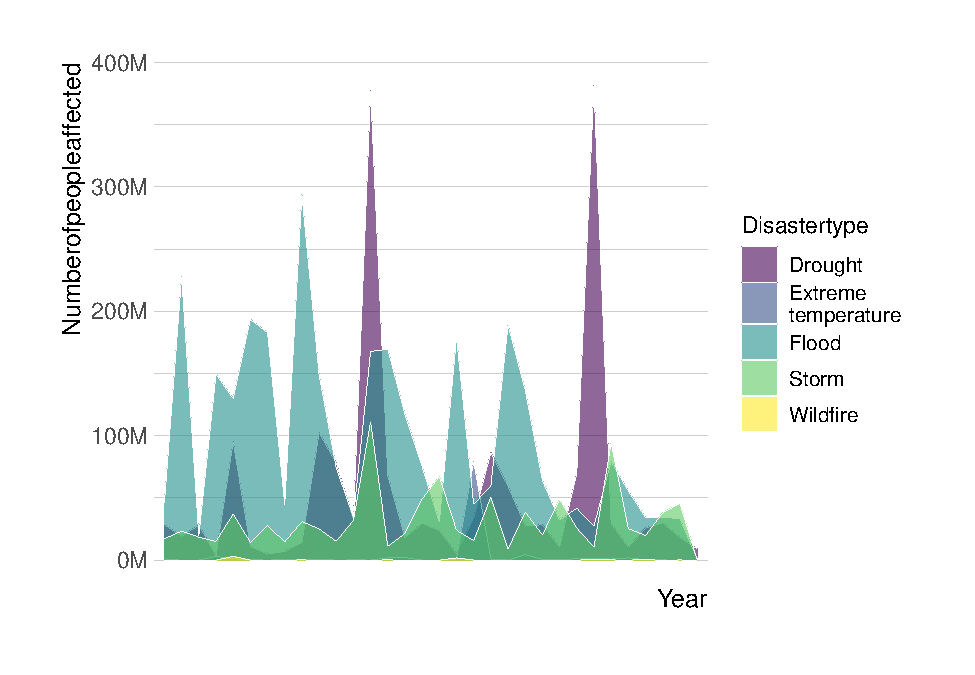
\includegraphics{em-dat-visualizations_files/figure-latex/plot disasters over time-1}

\begin{Shaded}
\begin{Highlighting}[]

\NormalTok{ggplot2}\SpecialCharTok{::}\FunctionTok{ggsave}\NormalTok{(}\FunctionTok{here}\NormalTok{(}\StringTok{"images"}\NormalTok{, }\StringTok{"vulnerability{-}01.svg"}\NormalTok{), }
    \AttributeTok{device =} \StringTok{"svg"}\NormalTok{, }\AttributeTok{dpi =} \DecValTok{300}\NormalTok{)}

\FunctionTok{rm}\NormalTok{(em\_dat)}
\end{Highlighting}
\end{Shaded}

\hypertarget{export-as-an-r-script-for-future-use}{%
\section{Export as an R script for future
use}\label{export-as-an-r-script-for-future-use}}

Only run this chunk manually once within the .Rmd file. It produces an
error when knitting it as a whole because of chunk label duplicates. As
of May 12, 2021, there hasn't been a viable solution to run the code
below when as part of the knitting process.

\begin{Shaded}
\begin{Highlighting}[]
\NormalTok{knitr}\SpecialCharTok{::}\FunctionTok{purl}\NormalTok{(}\StringTok{"em{-}dat{-}visualizations.Rmd"}\NormalTok{, }
    \StringTok{"em{-}dat{-}visualizations.R"}\NormalTok{)}
\NormalTok{knitr}\SpecialCharTok{::}\FunctionTok{write\_bib}\NormalTok{(}\FunctionTok{.packages}\NormalTok{(), }\StringTok{"packages.bib"}\NormalTok{)}
\end{Highlighting}
\end{Shaded}

\hypertarget{software-used}{%
\section*{Software used}\label{software-used}}
\addcontentsline{toc}{section}{Software used}

\hypertarget{refs}{}
\begin{CSLReferences}{1}{0}
\leavevmode\vadjust pre{\hypertarget{ref-R-janitor}{}}%
Firke, Sam. \emph{Janitor: Simple Tools for Examining and Cleaning Dirty
Data}, 2021. \url{https://github.com/sfirke/janitor}.

\leavevmode\vadjust pre{\hypertarget{ref-R-viridis}{}}%
Garnier, Simon. \emph{Viridis: Default Color Maps from Matplotlib},
2021. \url{https://CRAN.R-project.org/package=viridis}.

\leavevmode\vadjust pre{\hypertarget{ref-R-viridisLite}{}}%
---------. \emph{viridisLite: Colorblind-Friendly Color Maps (Lite
Version)}, 2021. \url{https://CRAN.R-project.org/package=viridisLite}.

\leavevmode\vadjust pre{\hypertarget{ref-R-here}{}}%
Müller, Kirill. \emph{Here: A Simpler Way to Find Your Files}, 2020.
\url{https://CRAN.R-project.org/package=here}.

\leavevmode\vadjust pre{\hypertarget{ref-R-base}{}}%
R Core Team. \emph{R: A Language and Environment for Statistical
Computing}. Vienna, Austria: R Foundation for Statistical Computing,
2021. \url{https://www.R-project.org/}.

\leavevmode\vadjust pre{\hypertarget{ref-R-hrbrthemes}{}}%
Rudis, Bob. \emph{Hrbrthemes: Additional Themes, Theme Components and
Utilities for Ggplot2}, 2020.
\url{http://github.com/hrbrmstr/hrbrthemes}.

\leavevmode\vadjust pre{\hypertarget{ref-ggplot22016}{}}%
Wickham, Hadley. \emph{Ggplot2: Elegant Graphics for Data Analysis}.
Springer-Verlag New York, 2016. \url{https://ggplot2.tidyverse.org}.

\leavevmode\vadjust pre{\hypertarget{ref-R-stringr}{}}%
---------. \emph{Stringr: Simple, Consistent Wrappers for Common String
Operations}, 2019. \url{https://CRAN.R-project.org/package=stringr}.

\leavevmode\vadjust pre{\hypertarget{ref-R-readxl}{}}%
Wickham, Hadley, and Jennifer Bryan. \emph{Readxl: Read Excel Files},
2019. \url{https://CRAN.R-project.org/package=readxl}.

\leavevmode\vadjust pre{\hypertarget{ref-R-ggplot2}{}}%
Wickham, Hadley, Winston Chang, Lionel Henry, Thomas Lin Pedersen,
Kohske Takahashi, Claus Wilke, Kara Woo, Hiroaki Yutani, and Dewey
Dunnington. \emph{Ggplot2: Create Elegant Data Visualisations Using the
Grammar of Graphics}, 2020.
\url{https://CRAN.R-project.org/package=ggplot2}.

\leavevmode\vadjust pre{\hypertarget{ref-R-dplyr}{}}%
Wickham, Hadley, Romain François, Lionel Henry, and Kirill Müller.
\emph{Dplyr: A Grammar of Data Manipulation}, 2021.
\url{https://CRAN.R-project.org/package=dplyr}.

\leavevmode\vadjust pre{\hypertarget{ref-R-scales}{}}%
Wickham, Hadley, and Dana Seidel. \emph{Scales: Scale Functions for
Visualization}, 2020. \url{https://CRAN.R-project.org/package=scales}.

\leavevmode\vadjust pre{\hypertarget{ref-R-extrafont}{}}%
Winston Chang. \emph{Extrafont: Tools for Using Fonts}, 2014.
\url{https://github.com/wch/extrafont}.

\end{CSLReferences}

\end{document}
